\documentclass[11pt]{article}

\usepackage{amsmath}
\usepackage{amssymb}

\usepackage{graphicx}
\usepackage{tikz}

\usepackage{ytableau}

\begin{document}

\begin{center}
{\bf Math 4990: Intro to combinatorics and graph theory \\
Fall 2020, Sam Hopkins \\
Final exam- Due Tuesday Dec. 15th}
\end{center}

{\bf Instructions}: There are 5 problems, worth 20 points each, totaling 100 points. This is an open book, open library, open notes, open web, take-home exam, but you are not allowed to to interact with anyone (including online forums) except for me, the instructor. As always, in order to earn points you need to carefully \emph{explain your answer}.

\begin{enumerate}

\item (20 points) Recall that we say a permutation $\pi \in S_n$ is a \emph{derangement} if $\pi(i)\neq i$ for all $i=1,\ldots,n$. Meanwhile, we say $\pi \in S_n$ is an \emph{involution} if $\pi^{2}(i)=i$ for all $i=1,\ldots,n$ (where $\pi^2(i)=\pi(\pi(i))$). Give a simple formula for the number of permutations in $S_n$ which are both derangements and involutions.

\item (20 points total; 10 points each)
\begin{enumerate}
\item How many paths in $\mathbb{R}^2$ from $(0,0)$ to $(50,100)$ taking steps of the form $(0,1)$ and $(1,0)$ are there?
\item  How many such paths are there which avoid passing through any of the 3 ``bad'' points
\[(10, 11), (20, 42), (30, 85)?\]
\end{enumerate}

\item (20 points) Let $n=2m$ be an even number, with $m > 1$. Let $G$ be the graph on $n$ vertices obtained from the complete graph $K_n$ by removing the edges of a Hamiltonian cycle. For example, in the cases $n=4$ and $n=6$, $G$ looks like the following:
\[ 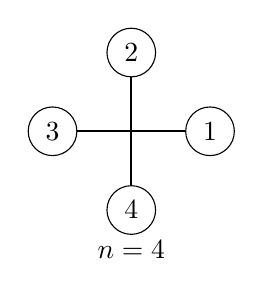
\begin{tikzpicture}
\node[draw, circle] (1) at (0:1) {1};
\node[draw, circle] (2) at (90:1) {2};
\node[draw, circle] (3) at (180:1) {3};
\node[draw, circle] (4) at (270:1) {4};
\node at (270:1.5) {$n=4$};
\draw[thick] (1)--(3);
\draw[thick] (2)--(4);
\end{tikzpicture} \qquad \qquad \qquad 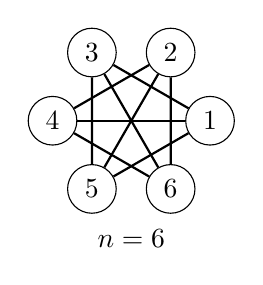
\begin{tikzpicture}
\node[draw, circle] (1) at (0:1) {1};
\node[draw, circle] (2) at (60:1) {2};
\node[draw, circle] (3) at (120:1) {3};
\node[draw, circle] (4) at (180:1) {4};
\node[draw, circle] (5) at (240:1) {5};
\node[draw, circle] (6) at (300:1) {6};
\node at (270:1.5) {$n=6$};
\draw[thick] (1)--(3)--(5)--(1);
\draw[thick] (2)--(4)--(6)--(2);
\draw[thick] (1)--(4);
\draw[thick] (2)--(5);
\draw[thick] (3)--(6);
\end{tikzpicture} \]
What is the chromatic number of $G$?
\end{enumerate}

\pagebreak

\begin{enumerate}
\setcounter{enumi}{3}

\item (20 points) The student newspaper of your school has a certain number of sports reporters: Sam, Emily, Lauren, .... The university plays a certain number of sports: Basketball, Soccer, Hockey, .... Each sports reporter is asked to list which sports they would be interested in covering. You are not told the number of reporters nor the number of sports. But what you do know is that:
\begin{itemize}
\item each reporter lists exactly 3 sports they are interested in covering;
\item and each sport has exactly 3 reporters who listed that sport.
\end{itemize}
Explain how you know that there is a way of assigning reporters to sports they listed, so that each reporter is assigned exactly one sport and each sport has exactly one reporter assigned to it.

\item (20 points) Your friend hands you a convex polyhedron in $\mathbb{R}^3$ which has triangular and hexagonal faces (and no other kinds of faces), and for which every vertex belongs to three edges. How many triangular faces must this polyhedron have? \\
{\bf Hint}: find various equations that relate the numbers $v$, $e$, $f$, $t$, $h$ of vertices, edges, faces, triangular faces, hexagonal faces, respectively.
\end{enumerate}

\end{document}
